% =====================================================================
%  monolito.tex  --  PUNTO DE PARTIDA DE LA PRÁCTICA
%  Taller "LaTeX con IA"  ·  Grupo Universitario de Informática (UVa)
% =====================================================================
%  Es la plantilla de entregables de la UVa (Template.tex) rellenada
%  con un poco de contenido. Todo está en un único fichero y tiene los
%  problemas típicos de una plantilla que se copia de proyecto en
%  proyecto. El preámbulo es el de la plantilla original; solo se ha
%  corregido la llave que faltaba en \title (ver [PROBLEMA 1]).
%
%  OBJETIVO: llevarlo a la estructura de ../01_solucion en 3 pasos.
%    PASO 1  Modularizar   -> diseño en styles/mistilo.sty,
%                             contenido en capitulos/, portada como comando
%    PASO 2  Bibliografía  -> thebibliography manual  =>  bib/refs.bib
%    PASO 3  Profesionalizar -> cabeceras, títulos, enlaces y cajas
%    PASO 4  Figuras         -> vectorizar con Inkscape (inkscape_guia.md)
%
%  Los comentarios [PROBLEMA n] señalan lo que hay que arreglar.
%  Las imágenes están en la carpeta Recursos/.
%  Compilar con:  pdflatex monolito.tex   (dos pasadas)
%
%  GUÍA DE LECTURA PARA QUIEN EMPIEZA
%  Un documento LaTeX tiene dos zonas:
%    1) PREÁMBULO: desde \documentclass hasta \begin{document}.
%       Aquí se carga el idioma, los paquetes y se define el diseño.
%       No se imprime nada.
%    2) CUERPO: entre \begin{document} y \end{document}.
%       Es lo que se ve en el PDF: portada, índice, secciones...
%  Convenciones:
%    - Una línea que empieza por %  es un comentario (LaTeX la ignora).
%    - \comando{argumento}: el comando actúa sobre lo que va entre llaves.
%    - \usepackage{x} carga el paquete "x" (extiende LaTeX).
%
%  ORDEN RECOMENDADO DE TRABAJO
%    a) Compila tal cual y mira el PDF resultante.
%    b) Lee los [PROBLEMA n] en orden y resuélvelos de uno en uno.
%    c) Compila tras CADA cambio: si algo falla, sabrás cuál fue.
%    d) Si dudas, compara con la carpeta 01_solucion.
% =====================================================================

% Clase de documento: define la estructura base. "article" divide en
% \section; [10pt] es el tamaño de letra.
\documentclass[10pt]{article}

% Idioma y codificación
% inputenc deja escribir tildes y ñ; babel[spanish] traduce los textos
% automáticos ("Índice", "Tabla"...) y ajusta la separación silábica.
\usepackage[utf8]{inputenc}
\usepackage[spanish]{babel}

% Márgenes: geometry define el tamaño de los márgenes de la página.
\usepackage{geometry}
\geometry{top=2.5cm, bottom=2.5cm, left=2.5cm, right=2.5cm}

% ---------- [PROBLEMA 2] Paquetes duplicados o redundantes ----------
% graphicx ya incluye lo necesario de graphics, y listings se carga
% dos veces. No da error, pero es ruido que se arrastra de plantilla
% en plantilla.
\usepackage{graphicx}
\usepackage{graphics}
\usepackage{wrapfig}
\usepackage{float}
\usepackage{amssymb}

% Listings: paquete para mostrar código con formato. xcolor permite
% usar colores; caption y capt-of personalizan los pies de figura/tabla.
\usepackage{listings}
\usepackage{xcolor}
\usepackage{caption}
\usepackage{capt-of}
\lstdefinestyle{terminal}{
	backgroundcolor=\color{gray!10},
	basicstyle=\ttfamily\small,
	keywordstyle=\color{blue},
	commentstyle=\color{gray},
	frame=single,
	columns=fullflexible,
	morecomment=[l]{//}
}
\usepackage{listings}   % <- repetido
\lstset{
	inputencoding=utf8,
	extendedchars=true,
	literate={á}{{\'a}}1 {é}{{\'e}}1 {í}{{\'i}}1 {ó}{{\'o}}1 {ú}{{\'u}}1 {ñ}{{\~n}}1
}

% ---------- [PROBLEMA 3] Enlaces con instrucciones contradictorias ----------
% hidelinks los oculta, pero \hypersetup los vuelve a pintar de colores
% llamativos (blue, magenta, cyan). Elegimos UNA política y un color
% de acento coherente con el resto del documento.
\usepackage[hidelinks]{hyperref}
\hypersetup{
	colorlinks=true,
	linkcolor=blue,
	filecolor=magenta,
	urlcolor=cyan,
}

% Encabezados y pies de página (fancyhdr).
% Aquí solo se coloca el número de página abajo a la derecha.
\usepackage{fancyhdr}
\pagestyle{fancy}
\fancyhf{}
\fancyfoot[R]{\thepage}

% Formato de títulos (titlesec): cómo se ven \subsection y \subsubsection.
% Observa que \section NO está personalizada y queda con el estilo por defecto.
\usepackage{titlesec}
\titleformat{\subsection}{\normalfont\large\bfseries}{\hspace{1em}\thesubsection}{1em}{}
\titleformat{\subsubsection}{\normalfont\normalsize\bfseries}{\hspace{2em}\thesubsubsection}{1em}{}

% ---------- [PROBLEMA 1] Datos de la portada ----------
% En la plantilla original faltaba una llave "}" al cerrar \title y el
% documento no compilaba. Aquí ya está corregido: ¡conviene saber
% leer el error y no solo pedírselo a la IA!
\title{\textbf{Título del entregable}}
\author{\textbf{\small Nombre Apellido}}
\date{}

\makeatletter
\let\thetitle\@title
\let\theauthor\@author
\let\thedate\@date
\makeatother

% Color de acento (se usará en cajas)
% \definecolor crea un color con nombre a partir de su código HTML
% (6 cifras hexadecimales). Después se usa como \color{acento}.
\definecolor{acento}{HTML}{3F6FB5}

\begin{document}

	% ---------- [PROBLEMA 4] Portada incrustada en el documento ----------
	% Titulación, mención y ruta del logo están escritos a mano. Para
	% cada entregable nuevo hay que editar el cuerpo del documento.
	% PASO 1: convertirla en un comando \makeportada definido en el .sty.
	\begin{titlepage}
		\centering
		
\includegraphics[scale=0.3]{Recursos/UVA-3881270087.pdf}\\[0.5cm]
		\rule{\linewidth}{0.2mm}\\[0.4cm]
		{\huge\bfseries \thetitle}\\
		\rule{\linewidth}{0.2mm}\\[1.5cm]
		{\Large\bfseries Ingeniería informática}\\[0.3cm]
		{\Large\bfseries Tecnologías de la información y la comunicación}\\[1cm]
		{\Large \theauthor}\\[1.5cm]
		{\Large \thedate}
	\end{titlepage}

	% \renewcommand{\contentsname}{Índice}: cambia el título del índice.
	% \tableofcontents genera el índice a partir de las secciones.
	% \newpage fuerza un salto de página.
	\renewcommand{\contentsname}{Índice}
	\tableofcontents
	\newpage

% =====================================================================
%  SECCIÓN 1  ->  debería ir a  capitulos/01_intro.tex
% =====================================================================
\section{Introducción}

La programación paralela es hoy una herramienta cotidiana, pero escribir
código paralelo eficiente y portable sigue siendo difícil. Una línea de
trabajo de la Universidad de Valladolid propone describir los programas
con especificaciones de alto nivel y dejar que un compilador modular
genere el código final~\cite{gonzalez2011trasgo}.
% \cite{clave} inserta una cita. La clave debe coincidir con la de un
% \bibitem (aquí, al final) o, tras el PASO 2, con una entrada de refs.bib.
% El símbolo ~ es un espacio que impide un salto de línea antes de la cita.

% [PROBLEMA 5] Caja de aviso hecha "a mano" con \fcolorbox y copiada
% varias veces. PASO 3: sustituirla por un entorno tcolorbox "aviso".
\medskip
\noindent\fcolorbox{acento}{acento!8}{%
  \parbox{0.94\textwidth}{\textbf{Aviso.} Este documento es solo un
  ejemplo para el taller: las referencias son reales, el resto es
  ficticio.}}
\medskip

% \subsection crea una subsección numerada (1.1). \ref{sec:datos} se
% sustituye por el número de la sección que lleva \label{sec:datos}.
\subsection{Estructura del informe}
La sección~\ref{sec:datos} describe un formato binario para publicar
grandes conjuntos de datos enlazados~\cite{fernandez2013hdt} y
presenta una tabla resumen.

% =====================================================================
%  SECCIÓN 2  ->  debería ir a  capitulos/02_datos.tex
% =====================================================================
\section{Datos enlazados a gran escala}
\label{sec:datos}

El formato \emph{HDT} divide un conjunto de datos RDF en tres
componentes: cabecera, diccionario y tripletas~\cite{fernandez2013hdt}.
Esa separación es, en el fondo, la misma idea que aplicamos hoy a
LaTeX: \textbf{dividir en módulos con una responsabilidad clara}.

% Entorno table: crea una tabla numerada con pie. [H] = colócala justo aquí.
% tabular{lll} = tres columnas alineadas a la izquierda; & separa
% columnas, \\ termina la fila y \hline dibuja una línea.
\begin{table}[H]
  \centering
  \begin{tabular}{lll}
    \hline
    \textbf{Componente} & \textbf{Contenido} & \textbf{Función} \\
    \hline
    Header     & Metadatos        & Describe el conjunto de datos \\
    Dictionary & Cadenas de texto & Evita repetirlas \\
    Triples    & Estructura       & Representa el grafo \\
    \hline
  \end{tabular}
  \caption{Los tres componentes de HDT.}
  \label{tab:hdt}
\end{table}

% [PROBLEMA 6] Tabla con \hline: líneas verticales de impresión pobre
% y sin espaciado. PASO 3: pedirle a la IA que la pase a booktabs.

% [PROBLEMA 8] Figura en mapa de bits (PNG de baja resolución): se ve
% borrosa al ampliar o imprimir. PASO 4: vectorizarla con Inkscape,
% guardar el PDF en Recursos/ y cambiar la extensión. Ver inkscape_guia.md.
\begin{figure}[H]
  \centering
  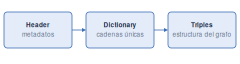
\includegraphics[width=0.8\linewidth]{Recursos/hdt_esquema.png}
  \caption{Esquema de HDT (versión en mapa de bits).}
  \label{fig:hdt}
\end{figure}

La figura~\ref{fig:hdt} y la tabla~\ref{tab:hdt} resumen la idea. Aquí tienes el mismo aviso,
copiado a mano por segunda vez:

\medskip
\noindent\fcolorbox{acento}{acento!8}{%
  \parbox{0.94\textwidth}{\textbf{Aviso.} Cuando copies y pegues un
  bloque por tercera vez, es hora de convertirlo en un entorno.}}
\medskip

% =====================================================================
%  BIBLIOGRAFÍA  ->  debería ser bib/refs.bib + biblatex
% =====================================================================
% \begin{thebibliography} es la forma ANTIGUA de escribir la bibliografía.
% Cada \bibitem{clave} es una entrada; {9} indica el ancho de la numeración.
% [PROBLEMA 7] Bibliografía escrita a mano: sin formato automático,
% imposible cambiar de estilo (IEEE, APA...) y propensa a erratas.
% PASO 2: crear bib/refs.bib y usar \printbibliography.
\begin{thebibliography}{9}

\bibitem{gonzalez2011trasgo}
A.~Gonz{\'a}lez-Escribano y D.~R. Llanos,
``Trasgo: a nested-parallel programming system,''
\textit{The Journal of Supercomputing}, vol.~58, n.º~2, pp.~226--234, 2011.

\bibitem{fernandez2013hdt}
J.~D. Fern{\'a}ndez, M.~A. Mart{\'i}nez-Prieto, C.~Guti{\'e}rrez,
A.~Polleres y M.~Arias,
``Binary RDF representation for publication and exchange (HDT),''
\textit{Journal of Web Semantics}, vol.~19, pp.~22--41, 2013.

\end{thebibliography}

\end{document}
